%template1.tex
%The following LaTeX source file represents the simplest kind of slide presentation; no overlays, no included graphics. Substitute your favorite style for ``pascal''. To create the PDF file template1.pdf, (1) be sure to use the prosper class, then (2) execute the command latex template1.tex, and (3) the command dvipdf template1.dvi.

%%%%%%%%%%%%%%%%%%%%%%%%%%%%%%% template1.tex %%%%%%%%%%%%%%%%%%%%%%%%%%%%%%%%%%%
\documentclass[a4paper,blends,pdf,colorBG,slideColor]{prosper}
% definitions for slides for CSC544
% Lutz Hamel, (c) 2007

\hypersetup{pdfpagemode=FullScreen}

\usepackage{times}
\usepackage{latexsym}
\usepackage{alltt}
\usepackage{booktabs}
\usepackage{amsmath}
\usepackage{amsopn}
\usepackage{amsfonts}
\usepackage{amssymb}
%\usepackage[usenames]{color}

\def\sign{\qopname\relax{no}{sign}}
\def\argmax{\qopname\relax{no}{argmax}}
\def\argmin{\qopname\relax{no}{argmin}}

\newcommand{\grad}{\ensuremath{\nabla}} 
\newcommand{\loss}{\ensuremath{{\cal L}}}
\newcommand{\err}{\mbox{err}}
\newcommand{\mse}{\mbox{mse}}
\newcommand{\acc}{\mbox{acc}}
\newcommand{\Integer}{\ensuremath{\mathbb{N}}}
\newcommand{\size}[1]{{|{#1}|}}
\newcommand{\Rnspace}[1]{\ensuremath{\mathbb{R}^{#1}}}
\newcommand{\Real}{\ensuremath{\mathbb{R}}}
\newcommand{\mytt}[1]{{\small\tt{#1}}}
\newcommand{\textemph}[1]{{\em #1}}
\newcommand{\suchthat}{\mid}
\newcommand{\orbar}{\;|\;}
\newcommand{\bs}[1]{\begin{slide}{#1}\ptsize{8}}
\newcommand{\es}{\end{slide}}
\newcommand{\co}{\,\colon\;}
\newcommand{\pair}[2]{\ensuremath{( {#1}, {#2} )}}
\newcommand{\model}[1]{\hat{#1}}
\newcommand{\ul}[1]{{\bf\em #1}}
\newcommand{\ol}{\overline}
\newcommand{\definition}[1]{{\bf Definition: }{\em #1}}
\newcommand{\example}[1]{{\bf Example: }{#1}}
\newcommand{\abs}[1]{|{#1}|}
\newcommand{\mytab}{\makebox[.1in]{}}

\newcommand{\fdef}[1]{
\begin{center}
\fbox{
\begin{minipage}{3.5in}
{\bf Definition:}
{#1}
\end{minipage}
}
\end{center}
}

\newcommand{\fframe}[1]{
\begin{center}
\fbox{
\begin{minipage}{3.5in}
{#1}
\end{minipage}
}
\end{center}
}

\newcommand{\nframe}[1]{
\begin{center}
\begin{minipage}{3.5in}
{#1}
\end{minipage}
\end{center}
}

\newenvironment{Rcode}
	{
		\scriptsize
		\begin{quote}
		\begin{alltt}
	}
	{
		\end{alltt}
		\end{quote}
	}




\begin{document}

\bs{Maximum Margin Classifiers}

\fframe{
{\bf Proposition:} (Maximum Margin Classifier)
Given a linearly separable training set 
\begin{equation*}
D = \{(\ol{x}_1,y_1),(\ol{x}_2,y_2),\ldots,(\ol{x}_l,y_l)\} \subseteq \Rnspace{n} \times \{+1,-1\},
\end{equation*}
we can compute a maximum margin  decision surface $\ol{w}^*\bullet\ol{x} = b^*$ with an optimization,
\begin{equation*}
\min \phi(\ol{w},b) = \min_{\ol{w},b}\frac{1}{2}\ol{w}\bullet\ol{w}
\end{equation*}
subject to the constraints,
\begin{equation*}
\ol{w}\bullet(y_i \ol{x}_i)\ge 1+ y_i b  \mbox{\hspace{.2in}\rm for all } (\ol{x}_i,y_i)\in D. 
\end{equation*}
}
\es

\bs{Maximum Margin Classifiers}

\vspace{.5in}
\begin{center}
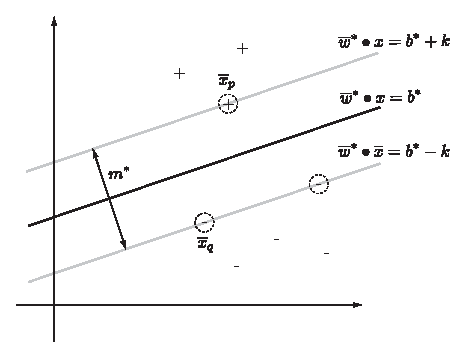
\includegraphics[height=45mm]{figures/fig06-05.eps}
\end{center}
\es


\bs{Convex Optimization}
Our objective function is convex,
\begin{equation*}
\phi(\ol{w},b) =  \frac{1}{2}\ol{w}\bullet\ol{w} = \frac{1}{2}(w_1^2 + \ldots + w_n^2),
\end{equation*}

\vspace{.2in}
\begin{minipage}{2in}
%\begin{center}
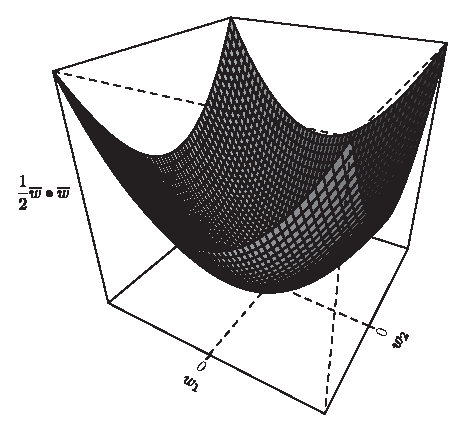
\includegraphics[height=45mm]{figures/fig06-07.eps}
%\end{center}
\end{minipage}
\begin{minipage}{2in}
Here $\ol{w}\in \Rnspace{2}$.
\end{minipage}
\es

\bs{Quadratic Programming - QP}
A {\em quadratic program} is a general convex optimization problem of the form
\begin{equation*}
\ol{w}^* =  \argmin_{\ol{w}} \left (\frac{1}{2} \ol{w}^T {\mathbf Q}\; \ol{w} - \ol{q}\bullet\ol{w}\right ),
\end{equation*}
subject to the constraints
\begin{equation*}
\label{eq;constraint-matrix}
{\mathbf X}^T\ol{w} \ge \ol{c}.
\end{equation*}
Here, $\mathbf Q$ is an $n\times n$ matrix, $\mathbf X$ is an $l\times n$ matrix, the vectors
$\ol{w}^*$, $\ol{w}$, $\ol{q}$ are $n$-dimensional vectors, and the vector $\ol{c}$ is an
$l$-dimensional vector. \footnote{I have written the quadratic program in terms of $\ol{w}$;
in the literature a different letter would typically be used for the optimization variable.}

In software packages this is usually given as function of the form,
\begin{equation*}
\ol{w}^* = \mbox{\it solve}({\mathbf Q}, \ol{q}, {\mathbf X}, \ol{c}).
\end{equation*}
\vspace{.2in}

\es

\bs{Quadratic Programming - QP}
In order to bring the generalized quadratic program into a form that we can use
for our maximum margin optimization we let 
\begin{align*}
{\mathbf Q}&={\mathbf I},\\
\intertext{and} 
\ol{q} &= \ol{0},
\end{align*}
then
\begin{equation*}
\ol{w}^* =  \argmin_{\ol{w}} \left (\frac{1}{2} \ol{w}^T {\mathbf I}\; \ol{w} - \ol{0}\bullet \ol{w} \right )= \argmin_{\ol{w}} \left ( \frac{1}{2}\ol{w}\bullet\ol{w} \right ),
\end{equation*}

\es

\bs{Quadratic Programming - QP}
Next, let us look at the original constraints,
\begin{equation*}
(y_i \ol{x}_i)\bullet\ol{w} \ge 1+ y_i b,
\end{equation*}
for all $(\ol{x}_i, y_i) \in D$ with $i = 1,\ldots, l$ and $\ol{x}_i = (x_i^1\ldots,x_i^n)$. 

We have to rewrite these into the matrix form,
\begin{equation*}
{\mathbf X}^T\ol{w} \ge \ol{c},
\end{equation*}
with

\begin{minipage}{2in}
\begin{equation*}
{\mathbf X} = 
\left ( 
\begin{array}{ccccc}
y_1 x_1^1 & \cdots & y_i x_i^1 &\cdots &y_l x_l^1 \\
\vdots & &\vdots&&\vdots \\
y_1 x_1^n& \cdots & y_i x_i^n &\cdots & y_l x_l^n
\end{array}
\right )
\end{equation*}
\end{minipage}
\begin{minipage}{2in}
\begin{equation*}
\ol{c} = 
\left (
\begin{array}{c}
1 + y_1 b\\
1 + y_2 b\\
\vdots\\
1 + y_l b 
\end{array}
\right )
\end{equation*}
\end{minipage}

\vspace{.2in}
{\bf Observation:} $b$ is now a free variable in the optimization problem, its value is not computed
by the optimization algorithm but must be set by the user.
\es

\bs{Quadratic Programming - QP}
\fframe{
{\bf Proposition:} (Quadratic Programming)
Given a linearly separable training set 
\begin{equation*}
D = \{(\ol{x}_1,y_1),(\ol{x}_2,y_2),\ldots,(\ol{x}_l,y_l)\} \subseteq \Rnspace{n} \times \{+1,-1\},
\end{equation*}
then we can compute a maximum margin decision surface $\ol{w}^*\bullet\ol{x} = b^*$ 
with a quadratic programming approach that solves the generalized optimization problem,
\begin{equation*}
(\ol{w}^*,b^*) =   \argmin_{\ol{w},b} \left (\frac{1}{2} \ol{w}^T {\mathbf Q}\; \ol{w} - \ol{q}\bullet \ol{w}\right ),
\end{equation*}
subject to the constraints
\begin{equation*}
{\mathbf X}^T\ol{w} \ge \ol{c},
\end{equation*}
with ${\mathbf Q} = {\mathbf I}$, $\ol{q} = \ol{0}$, and where $\mathbf X$, and $\ol{c}$ are constructed 
according to the previous discussion.
}
\es

\bs{QP - Algorithm}

\begin{center}
\fbox{
\begin{minipage}{3in}
{\small
{\bf let} $D = \{(\ol{x}_1,y_1), (\ol{x}_2,y_2),\dots,(\ol{x}_l,y_l)\} \subset \Rnspace{n} \times \{+1, -1\}$\\
$r \leftarrow \max \{ \abs{\ol{x}} \mid (\ol{x},y)\in D \}$\\
$q \leftarrow 1000$\\
{\bf let} $\ol{w}^*$ {\rm and} $b^*$ {\rm be undefined}\\
{\rm construct $\mathbf X$}\\
{\bf for each} $b \in [-q,q]$ {\bf do}\\
\mytab {\rm construct $\ol{c}$}\\
\mytab $\ol{w} \leftarrow \mbox{\it solve}({\mathbf I}, \ol{0},{\mathbf X}, \ol{c})$\\
\mytab {\bf if} ($\ol{w}$ {\rm is defined} {\bf and} $\ol{w}^*$ {\rm is undefined}) {\bf or}\\
\mytab\mytab ($\ol{w}$ {\rm is defined} {\bf and} $\abs{\ol{w}} < \abs{\ol{w}}^*$) {\bf then}\\
\mytab\mytab $\ol{w}^*$ $\leftarrow$ $\ol{w}$ \\
\mytab\mytab ${b^*}$ $\leftarrow$ $b$ \\
\mytab {\bf end if}\\
{\bf end for}\\
{\bf if} $\ol{w}^*$ {\rm is undefined} {\bf then} {\bf stop} {\rm constraints not satisfiable}\\
{\bf else if}  $\abs{\ol{w}}^* > q/r$ {\bf then} {\bf stop} {\rm bounding assumption of $\abs{\ol{w}}$ violated}\\
{\bf end if}\\
{\bf return} $(\ol{w}^*,b^*)$ 
}
\end{minipage}
}
\end{center}
\es



\bs{QP - Example}
\small
Let \[D = \{\pair{(1,6)}{-1},\pair{(3,7)}{-1},\pair{(1,4)}{+1},\pair{(2,1)}{+1}\}\] be the training set and let
\begin{equation*}
\ol{w}^* = \mbox{\it solve}({\mathbf Q}, \ol{q}, {\mathbf X}, \ol{c}),
\end{equation*}
be a call to the solver, then

\begin{minipage}{1.5in}
\[
{\mathbf X} = \left [
\begin{array}{cccc}
-1 & -3 & 1 & 2 \\
-6 & -7 & 4 & 1
\end{array}
\right ]
\]
\end{minipage}
\begin{minipage}{1.5in}
\[
\ol{c} = \left [
\begin{array}{c}
1 - b\\
1 - b\\
1 + b\\
1 + b
\end{array}
\right ]
\]
\end{minipage}

\begin{minipage}{1.5in}
\[
{\mathbf Q} = \left [
\begin{array}{cc}
1 & 0  \\
0 & 1
\end{array}
\right ]
\]
\end{minipage}
\begin{minipage}{1.5in}
\[
\ol{q} = \left [
\begin{array}{c}
0\\
0
\end{array}
\right ]
\]
\end{minipage}

\es

\bs{QP - Free Parameter}

{\bf Observation:} Our optimization problem has a free parameter, the offset term $b$. 
Notice also that the constraints are dependent on this term.  That is we need to
pick $b$ in such a way that the constraints are consistent.  In other words, we need to
pick $b$ in such a way that the quadratic solver can actually find a minimum $\ol{w}$.

What are reasonable values for $b$ to try?
\es

\bs{QP - Free Parameter}
First observation,
\begin{equation*}
\begin{array}{rcr}
b = \ol{w}\bullet\ol{x}&\Rightarrow&\\
b = \abs{\ol{w}}\abs{\ol{x}} \cos \gamma&\Rightarrow& (-1 \le \cos \gamma \le 1, \text{for all $\gamma$})\\
-  \abs{\ol{w}}\abs{\ol{x}} \le b \le  \abs{\ol{w}}\abs{\ol{x}}&\Rightarrow& (\abs{\ol{x}} \le r)\\
-  \abs{\ol{w}}r \le b \le  \abs{\ol{w}}r &\Rightarrow&
\end{array}
\end{equation*}
Second observation, $2r$ is the size of the largest margin and $\ol{w}$ is unbounded,
\begin{equation*}
\frac{2}{\abs{\ol{w}}} \le 2r\Rightarrow \frac{1}{r} \le \abs{\ol{w}}
\end{equation*}
Third observation, we bound $\ol{w}$,
\begin{equation*}
\frac{1}{r} \le \abs{\ol{w}} \le \frac{q}{r}
\end{equation*}
Finally, we use $\ol{w}=q/r$ in the equation above,
\begin{equation*}
-  \abs{\ol{w}}r \le b \le  \abs{\ol{w}}r \Rightarrow  -q \le b \le  q
\end{equation*}
\es


\end{document}
%%%%%%%%%%%%%%%%%%%%%%%%%%% end of template1.tex %%%%%%%%%%%%%%%%%%%%%%%%%%%%%%%%

